\RequirePackage{luatex85}
\documentclass[12pt]{article}
\usepackage[margin=0.5in, bottom=0.35in, columnsep=1.0in]{geometry}
\usepackage{graphicx, adjustbox, tikz-cd, amsmath, amssymb, multicol, lscape, mathtools, etoolbox}
\setlength\parindent{0pt}

\def\luamath#1{\edef\luamathresult{\directlua{tex.write("" .. #1)}}}
\pgfkeys{/pgf/number format/.cd, fixed, fixed zerofill, precision=4}
\newcommand\normal[1]{
	\pgfmathparse{#1 > 0 ? 1 : -1}%
	\edef\sign{\pgfmathresult}%
	\pgfmathparse{abs(#1)}%
	\edef\x{\pgfmathresult}%
	\luamath{(\sign+1)/2 - \sign
		*(2*3.141592653589793*2.718281828459045^(\x^2))^-0.5
		*(0.4361836/(1+0.33267*\x)
			- 0.1201676/(1+0.33267*\x)^2 
			+ 0.9372980/(1+0.33267*\x)^3
			)
		}
	\pgfmathparse{\luamathresult}
	\pgfmathroundto\pgfmathresult
	\xappto\NormalTable{& $\pgfmathresult$}
	}
\def\arraystretch{0.68}
\def\NormalTable{}%
\foreach \ab in {34,...,0}{
	\pgfmathparse{floor(\ab/10)} \pgfmathroundto\pgfmathresult \xdef\a{\pgfmathresult}
	\pgfmathparse{mod(\ab, 10)} \pgfmathroundto\pgfmathresult \xdef\b{\pgfmathresult}
	\xappto\NormalTable{$-\a.\b$}
	\foreach \c in {0, ..., 9}{\normal{-\ab/10-\c/100}}
	\xappto\NormalTable{& $-\a.\b$ \noexpand\\ }
	\ifnum\b=0 \xappto\NormalTable{&&&&&&&&&&{} \noexpand\\ } \else \fi
	}
\xappto\NormalTable{\noexpand\\[-4ex] }%
\foreach \ab in {0,...,34}{
	\pgfmathparse{floor(\ab/10)} \pgfmathroundto\pgfmathresult \xdef\a{\pgfmathresult}
	\pgfmathparse{mod(\ab, 10)} \pgfmathroundto\pgfmathresult \xdef\b{\pgfmathresult}
	\ifnum\b=0 \xappto\NormalTable{&&&&&&&&&&{} \noexpand\\ } \else \fi
	\xappto\NormalTable{$\a.\b$}
	\foreach \c in {0, ..., 9}{\normal{\ab/10+\c/100}}
	\xappto\NormalTable{& $\a.\b$ \noexpand\\ }
	}%

\begin{document}
\begin{landscape}
\pagestyle{empty}
\huge %\sf
Standard Normal table %Standard Normal Cumulative Distribution Function $F_Z$
\par\vspace{0.2in}\large\hfill
\begin{tikzcd}[column sep=3.5cm, row sep=-2mm]
	\text{\LARGE standard units}\quad
	\rar[leftrightarrow, "\text{\normalsize use table to convert}"]
	& \quad\text{\LARGE percentile rank}
	\\ \displaystyle\boldsymbol z\color{black} = \frac{x-\mu}\sigma\quad\,\,
	& \quad\boldsymbol{P(z \text{ or less})}
	\color{black} = \text{area left of }z
	\end{tikzcd}
\hfill\hfill~
$\smash{\begin{matrix}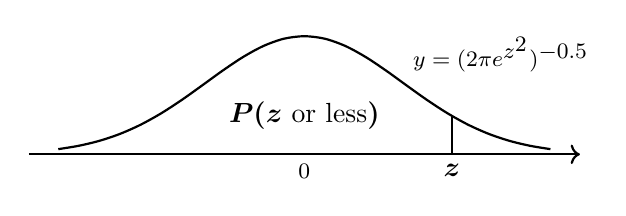
\begin{tikzpicture}[thick, yscale=1.5, xscale=1.25]
	\draw[smooth, domain=-2.5:2.5] plot (\x, {2.718^(-0.5*(\x*\x))});
	\draw (1, {2.718^-0.5}) node[above right, outer sep=0.4pt] (fZ) 
	{\footnotesize$\color{black} y=(2\pi e^{\textstyle z^{\textstyle2}})^{\textstyle-0.5}$};
	\draw (-2.8, 0) edge[->] (2.8, 0);
	\draw  (1.5,0) node[below] {$\boldsymbol z$} -- ++(up: {2.718^(-0.5*(1.5*1.5))});
	\draw (0,0) node[below, black, outer sep=0.4pt] {\footnotesize0};
	\draw (0, 0.33) node {$\boldsymbol{P(z\text{ or less})}$};
	\end{tikzpicture}\end{matrix}}$
\hfill~

\footnotesize
\begin{adjustbox}{angle=270}
\begin{tabular}{r@{\hspace{4.5mm}}
	*5{l @{\hspace{2.5mm}}}@{\hspace{-0.5mm}}*5{@{\hspace{2.5mm}}l}@{\hspace{2mm}}r}
& 0.00 & 0.01 & 0.02 & 0.03 & 0.04 & 0.05 & 0.06 & 0.07 & 0.08 & 0.09 \\
&&&&&&&&&&{} \\
$\mathllap\le{-}3.5\mathrlap0$ & 0.0001\\
\NormalTable
$\mathllap\ge3.5\mathrlap0$ & 0.0001\\
&&&&&&&&&&{} \\
& 0.00 & 0.01 & 0.02 & 0.03 & 0.04 & 0.05 & 0.06 & 0.07 & 0.08 & 0.09
\end{tabular}
\end{adjustbox}
\par\vfill\small
City University of New York / College of Staten Island / M Sunderland
\hfill\textcolor{black}{symmetry: $P(-z$ or less) = $1 - P(z$ or less)}
\end{landscape}
\end{document}